\section{AI Methods and Algorithms}  \normalfont

In this section, it is described the multiple algorithms and approaches that are relevant to the work presented in this thesis, and that were used and developed so far in the publications. First, we will give a brief introduction into the main two areas respectively, Evolutionary Computation (EC) and Machine Learning (ML), to then continue into the specific approaches used. When applicable, it will be highlighted what was developed as part of the publications.

\subsection{Evolutionary Computation}

% \begin{itemize}
%     \item Introduce evolutionary computation
%     \item evolutionary algorithms
%     \item evolutionary strategies
%     \item evolutionary mechanism: Selection, crossover, mutation, replacement
% \end{itemize}

% Evolutionary Computation, here we go!~\cite{eiben2007-introductionEC}. 

\acrfull{ec} is a subfield within~\acrshort{ai} inspired on Darwin's theory of evolution~\cite{darwin1859-originSpecies} and Darwinian principles of natural selection and evolution of population over generations to primary solve/optimize a problem or task, with the premise of ``survival of the fittest".~\acrshort{ec} is a family of population-based algorithms that focuses on searching a multidimensional space for solutions through executing an iterative refinement loop. The basic premise is that by having a set of individuals in an environment to be experienced or with tasks to be solved, arises competion that causes natural selection, which results in finding high-performing solutions.~\acrfull{ea} is a subset of~\acrshort{ec}, which applies a set of evolutionary mechanisms in the refinement cycle: \textit{selection}, \textit{variation operators}, \textit{evaluation}, and \textit{replacement}~\cite{eiben2007-introductionEC}.

A typical~\acrshort{ea} starts by \emph{creating} a set of random solutions in the multidimensional space and \emph{evaluates} them using some fitness function. Based on this measurement, solutions can be sorted and better candidates can be \emph{selected} to seed the next generation, and~\emph{variation operators} such as recombination or mutation can be applied to them to create a new set of candidates, i.e. the offspring. These solutions are once again~\emph{evaluated}, and compete against the current population to \emph{replace} them, and be part of the next generation. This process is repeated until a solution of sufficient quality is found, which ends the execution. A pseudocode of the~\acrshort{ea} loop is show in listing~\ref{alg:EA}. In such a loop, Eiben and Smith highlights two evolutionary mechanism as fundamental for continuously producing and encountering high-performing individuals as well as creating diversity. The~\emph{selection} mechanism increases the pressure on selecting high-performing individuals for variation, which ultimately would result in increasing the quality of the population. The~\emph{variation operator}, which vary individuals to produce candidate solutions, creates the necessary diversity; thus achieving novelty. 

Moreover, under the subset of~\acrshort{ea} there exist four main variants:~\emph{Genetic Algorithms},~\emph{Genetic Programming},~\emph{Evolution Strategies}, and~\emph{Evolutionary Programming}. However, their distinction is mainly on the encoding of the individuals, i.e., how each individual or solution is internally represented, which at the same time, limits what variant operators can be applied. For instance, Genetic Algorithms use genes encoded as finite strings while Evolution Strategies' individuals are represented as real-valued vectors where approaches such as Covariance Matrix Adaptation could be applied~\cite{fontaine2019covariance}. Genetic algorithms are used for the work presented in this thesis, as the content to be evolved (i.e., levels in a dungeon) is represented as a finite set of integers, and as such operators such as mutation and recombination through crossover can be applied.

\begin{figure}
    \centering
     \subfloat[Genotype\label{subfig-1:directGen}]{%
       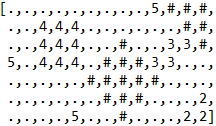
\includegraphics[width=0.45\textwidth]{figures/EC/directEncoding-gen2.png}
     }
     \hfill
     \subfloat[Phenotype\label{subfig-2:directPhen}]{%
       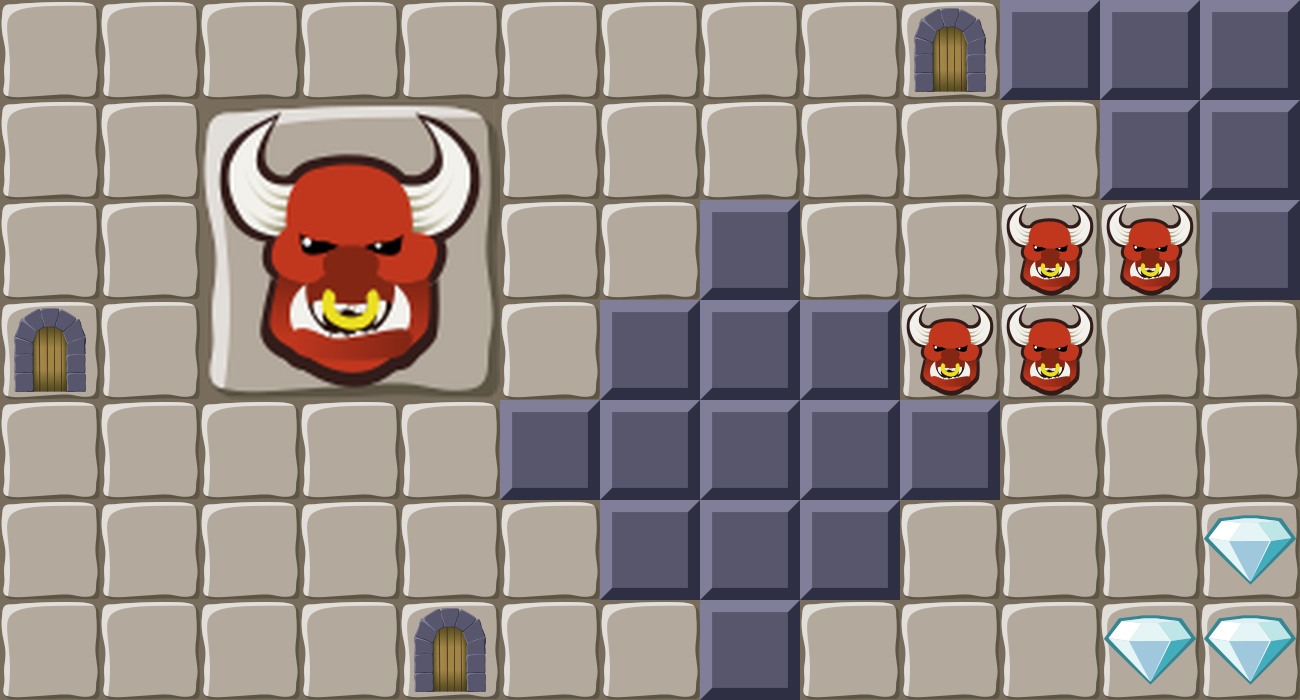
\includegraphics[width=0.45\textwidth]{figures/EC/directEncoding-phen.png}
     }
    
    \caption{Example of direct encoding}
    \label{fig:directENCOD}
\end{figure}

\subsubsection{Evolutionary Algorithm Components}

\paragraph{Representation}
Individuals (i.e. solutions) within a population have two representations: genotypes and phenotypes. \emph{Genotype} is the internal representation within the~\acrshort{ea} of the individual while \emph{Phenotype} is the ``translation" of the genotype when acting in the environment. For instance, humans genotypical representation is the DNA (genotype) while the body, brain, organs, etc. are the phenotypical representation. Such representation and translation is also called \emph{encoding}, which can fluctuate from direct to indirect encoding. Direct encoding refers that the genotype is mapped bit-by-bit to the phenotype, while indirect encoding refers to the opposite, the genotype is minimally encoded and its representation does not match the phenotype. To exemplify this, in the case of evolving tile-based rooms in a dungeon, a direct encoding could mean that the genotype is an array with integers each denoting a space in the room and the corresponding tile in the phenotype (shown in figure~\ref{fig:directENCOD}). A lesser direct encoding could have the genotype be an array that group together areas of the room and mark them as specific areas, or an even lesser let it just be a ruleset (such as in L-systems~\cite{Lindenmayer1996-LSystems,shaker2012evolving}) to create the levels. Encoding and representation of individuals is one of the main challenges in~\acrshort{ea} since the encoding can drastically change the evolutionary mechanisms and how the content is generated and explored~\cite{Ashlock2016-RepresentationsSearchBased,Clune2011-IndirectEncoding,Stanley2007-CPPN}.

\paragraph{Evaluation}

To assess the population and solutions, it is usually used a fitness function that estimates the quality of the solutions by testing some metrics that estimates and rank these solutions. Fitness functions are usually context-dependant and help solve the tasks at hand by using some representative heuristic of the task, for instance, if evolving levels in a game, quality can be measured in function of the tile distribution or the challenge vs. reward. However, objective-based functions might not be the best way of evaluating content as environments and tasks could be deceptive with a space filled with minimal optima, limiting the search; or diversity among the solutions might want to be rewarded rather than just ranking. Stanley and Lehman discuss such challenges with objective-based functions and proposed the use of divergent searches for stepping stones to solutions, with the aim of open-endedness~\cite{stanley2015-mythObjective}. More work and discussion on this is presented in section~\ref{sec:Backqd}.

\paragraph{Selection}

Selection is used to choose the parents of the next generation of candidate solutions; thus, it chooses which individuals will be applied the variation operators. Selection approaches are bias towards selecting high quality individuals, after all these ones are the ones with the best chances to generate better candidates. However, to counter greedy strategies and avoid getting stuck in local optima, lower-quality individuals still get a chance to be selected (with a similar idea to tabu-search). 
% There are three main approaches to selection: \emph{roulette}: , \emph{tournament}: , and \emph{ranking}:.

\paragraph{Variation Operators}

Once individuals from a population are selected, they are applied a set of variation operators to create candidates for the next generation. The operators might be \emph{Mutation} or recombination usually in the shape of crossover. Mutation is applied to a single individual with the aims of varying some genes from the genotype to create variation and diversity. For instance, if mutation is not applied, the~\acrshort{ea} is limited to the genes encountered in the initial population; if a key gene was not produced, the global optima might never be found. Common mutation operators are to swap a gene for another in the genotype, or randomly change a gene for a random value. Crossover requires at least two individuals that can, as the name indicates, cross their genes to form new candidates. Such is exemplified in figure~\ref{fig:crossoverEX}. The result of applying these operators to the selected parents is a set of candidate solutions (offspring) that are evaluated and compete against the current population for a place in the next generation.

\begin{figure}
\centerline{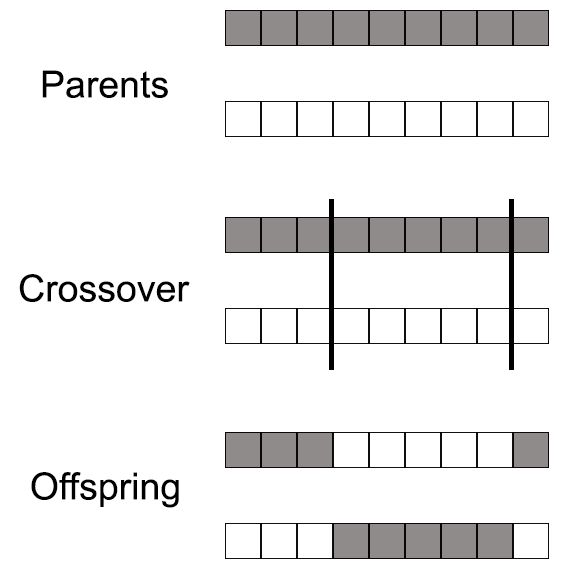
\includegraphics[width=0.5\textwidth]{figures/EC/crossover-example-bw.png}}
\caption{Example of the crossover variation operator
} \label{fig:crossoverEX}
\end{figure}

\paragraph{Replacement}

Replacement strategies mainly focus on replacing lower-quality individuals from the population for better candidates generated through the variation operators, hence, ``survival of the fittest". However, as it will be explain in section~\ref{sec:map-elites}, not all~\acrshort{ea} work the same. Some have local competition with individual with similar behavioral novelty~\cite{Lehman2011-NSLC}, other approaches have competition among phenotypical similars to preserve innovations encountered in the search space~\cite{Stanley2002-NEAT}.

% \begin{algorithm}
% \caption{Evolutionary Algorithm Loop}\label{alg:EA}
% \begin{algorithmic}
% \Procedure{EA}{}
% \State $POPULATION \gets RND\_SOLUTIONS$
% \State $EVALUATE$ each solution \textit{in} $POPULATION$
% % \State $a\gets b$
% % \Procedure{Euclid}{$a,b$}\Comment{The g.c.d. of a and b}
%   \State $r\gets a\bmod b$
%   \While{$r\not=0$}\Comment{We have the answer if r is 0}
%       \State $a\gets b$
%       \State $b\gets r$
%       \State $r\gets a\bmod b$
%   \EndWhile\label{euclidendwhile}
%   \State \textbf{return} $b$\Comment{The gcd is b}
% \EndProcedure
% \end{algorithmic}
% \end{algorithm}





% ~\acrshort{ec} is a family of population-based algorithms to solve tasks through a trial-and-error approach (i.e., try the solution, evaluates it, and try with something more appropriate), also called metaheuristic algorithms. In~\acrshort{ec}, the focus is 


% ~\acrfull{ea} are a 



% ~\acrshort{ec} are somewhat generic algorithms and the focus of the algorithm designer is to decide the repre

% To use~\acrshort{ec}, there are 

% \subsubsection{Feasible-Infeasible two-Population}

% \begin{itemize}
%     \item What is FI-2Pop
% \end{itemize}

% \subsubsection{Interactive Evolution}

% \begin{itemize}
%     \item simple not extensive text about IE \cite{Takagi2001-InteractiveEvo}
% \end{itemize}

\subsubsection{MAP-Elites} \label{sec:map-elites}

% \begin{itemize}
%     \item brief on QD since that was already introduced~\cite{Pugh2016}
%     \item present MAP-Elites and some of its variants~\cite{Mouret2015,Khalifa2018,cvt-mape2016,fontaine2019covariance,cluster-mape2017}'
%     \item but mostly focus 
% \end{itemize}

\acrlong{qd} algorithms are a relatively new family of algorithms that leverage in the strenghts of divergence and convergence search~\cite{Pugh2016}. One algorithm from this family is~\acrshort{mape}, which explores the space yielding a collection of solutions that are both high-performing and diverse. The main characteristics of~\acrshort{mape} are: 1) that it returns a collection of high-performing yet diverse solutions to address multiple wanted behavioral characteristics, for instance, robots that are able to move around and have a set of different behaviors and characteristics~\cite{Cully2015-qdRobotsAnimals}. 2) Using behavioral features as dimensions and discretising the space with cells, helps the algorithm illuminate the space, and control niches of individuals. and 3) By using these features and cells, the algorithm is able to substantially explore the space finding in the way a greater amount of solutions than in other approaches.~\acrshort{mape} has been extensively evaluated and resulted in a far superior approach to convergence search (i.e., objective-based) or divergence search (e.g. novelty search) alone, and other~\acrshort{qd} approaches such as~\acrshort{nslc}~\cite{Mouret2015}. 

\acrshort{mape} while superior to other approaches, its iterative cycle is not that different as the one presented earlier in this chapter. The main changes that~\acrshort{mape} introduce are: 1) instead of having one population, the~\acrshort{ea} uses cells; and 2) besides the fitness function to calculate the quality of individuals, it requires a set of behavioral feature dimensions to divide the space in cells and where individuals will be stored. In the vanilla version of~\acrshort{mape}, each cell contains one individual and as the search encounters new individuals within the same cell, the individual with higher-quality is kept and the other is disregarded. This way, the algorithm is able to preserve only high-quality solutions while retaining diverse solutions. 

Moreover, the algorithm is shown in Listing~\ref{alg:mape}, first initializes a collection of individuals that are evaluated with the fitness function and tested for their behavioral features to be placed in specific cells. Then random selection\footnote{Gravina et al. have experimented on using other selection approaches with beneficial and exciting results~\cite{Gravina2019-blendingNotionsDiversity}.} occurs on top of cells to pick individuals that then compete in a classical selection strategy (e.g., comparing fitness) to produce candidate solutions. Variation operators are applied to the selected parents and the offspring are evaluated with the fitness function and also tested for their behavioral features. Depending on the cell the offspring belong, they will need to compete if occupied with the current occupant or if unoccupied, the offspring is placed in the cell, and the cycle restarts. With such a simple algorithm,~\acrshort{mape} is able to encounter and return a collection of diverse and high-performing individuals. This is, firstly, due to the pressure in cells for high-performing individuals and secondly, due to retaining individuals in these multidimensional cells, where they might be completely different to another solution (e.g., have a complete different genotype) yet be as high-performing.


\begin{algorithm}
\begin{algorithmic}
\Procedure{MAP-Elites Algorithm (simple, default version)}{}
\State $(\mathcal{P} \leftarrow \emptyset, \mathcal{X} \leftarrow \emptyset)$
\For{iter $  = 1\to I$}
\If{iter $< G$} 
  \State $\mathbf{x'}\leftarrow $ random\_solution()  
\Else 
  \State $\mathbf{x}\leftarrow $ random\_selection($\mathcal{X}$) 
  \State $\mathbf{x'}\leftarrow $ random\_variation($\mathbf{x}$) 
\EndIf
\State $\mathbf{b'}\leftarrow $feature\_descriptor($\mathbf{x'}$) 
\State $p'\leftarrow $performance($\mathbf{x'}$) 
\If{$\mathcal{P}(\mathbf{b'})= \emptyset$ or $\mathcal{P}(\mathbf{b'})<p'$}
\State $\mathcal{P}(\mathbf{b'})\leftarrow p'$ 
\State $\mathcal{X}(\mathbf{b'})\leftarrow \mathbf{x'}$ 
\EndIf
\EndFor
\State \Return feature-performance map ($\mathcal{P}$ and $\mathcal{X}$)
\EndProcedure
\end{algorithmic}
\caption{Pseudocode description of the MAP-Elites Algorithm. Taken from~\cite{Mouret2015}.}
\label{alg:mape}
\end{algorithm}

%%UNCOMMENT FOR ADDING THE COMMENTS

% \begin{algorithm}
% \begin{algorithmic}
% \Procedure{MAP-Elites Algorithm (simple, default version)}{}
% \State $(\mathcal{P} \leftarrow \emptyset, \mathcal{X} \leftarrow \emptyset)$\Comment{\emph{Create an empty, $N$-dimensional map of elites:  \{solutions $\mathcal{X}$ and their performances $\mathcal{P}$\} }}
% \For{iter $  = 1\to I$} \Comment{\emph{Repeat for $I$ iterations.}}
% \If{iter $< G$} \Comment{\emph{Initialize by generating $G$ random solutions}}
%   \State $\mathbf{x'}\leftarrow $ random\_solution()  
% \Else \Comment{\emph{All subsequent solutions are generated from elites in the map}}
%   \State $\mathbf{x}\leftarrow $ random\_selection($\mathcal{X}$) \Comment{\emph{Randomly select an elite $x$ from the map $\mathcal{X}$}}
%   \State $\mathbf{x'}\leftarrow $ random\_variation($\mathbf{x}$) \Comment{\emph{Create $x'$, a randomly modified copy of $x$ (via mutation and/or crossover)} }
% \EndIf
% \State $\mathbf{b'}\leftarrow $feature\_descriptor($\mathbf{x'}$) \Comment{\emph{Simulate the candidate solution $x'$ and record its feature descriptor $\mathbf{b'}$}}
% \State $p'\leftarrow $performance($\mathbf{x'}$) \Comment{\emph{Record the performance $p'$ of $x'$}}
% \If{$\mathcal{P}(\mathbf{b'})= \emptyset$ or $\mathcal{P}(\mathbf{b'})<p'$}\Comment{\emph{If the appropriate cell is empty or its occupants's performance is $\leq p'$, then}}
% \State $\mathcal{P}(\mathbf{b'})\leftarrow p'$ \Comment{\emph{store the performance of $x'$ in the map of elites according to its feature descriptor $\mathbf{b'}$}}
% \State $\mathcal{X}(\mathbf{b'})\leftarrow \mathbf{x'}$ \Comment{\emph{store the solution $x'$ in the map of elites according to its feature descriptor $\mathbf{b'}$}}
% \EndIf
% \EndFor
% \State \Return feature-performance map ($\mathcal{P}$ and $\mathcal{X}$)
% \EndProcedure
% \end{algorithmic}
% \caption{A pseudocode description of the simple, default version of MAP-Elites.}
% \label{alg:mape}
% \end{algorithm}

Furthermore,~\acrshort{mape} have become popular and attractive due to all the abovementioned benefits and characteristics, which have not only spread it's use in many fields and many experiments, but also sparked many variations. The Constrained~\acrshort{mape} by Khalifa et al.~\cite{Khalifa2018} is the one this thesis relies on and have expanded. In their approach, they added populations in each cell rather than individuals, preserving even more solutions, and combined~\acrshort{mape} with~\acrshort{fi2pop}, which yielded two populations per cell, one driven by the fitness and the other driven by satisfying a set of constraints. Through this, they applied the same process as with the vanilla~\acrshort{mape} but per population (i.e., feasible and infeasible), which resulted in good and interesting results for the generation of bullet hells bosses.







% \subsubsection{Quality Diversity Algorithms}

% \begin{itemize}
%     \item brief, since we have already present most of the 
% \end{itemize}

% \paragraph{MAP-Elites}

\paragraph{Interactive Constrained MAP-Elites}

% \begin{itemize}
%     \item Present and discuss~\acrfull{icmape}.
% \end{itemize}

The~\acrfull{icmape}~\cite{alvarez2019empowering,Alvarez2020-ICMAPE} is the main algorithm developed in this thesis, which focuses on adapting the Constrained~\acrshort{mape} to be used in an~\acrshort{micc} system allowing designers to interact with it, and change non-intuitive aspects of~\acrshort{mape}. The main novel characteristics of~\acrshort{icmape} are:
% to be interacted by the designer. 

\begin{itemize}
    \item Adapting~\acrshort{mape} to be used to co-design levels by proposing suggestions in an~\acrshort{micc} system.
    \item Use of~\acrshort{mape} to create dungeons and adventure levels.
    \item Continuously adapting the fitness landscape and search space based on the designer's creation, which in turn, makes~\acrshort{mape} continuously adapting to a changing space.
    \item Customizable behavioral feature dimensions as part of the designer's ability to interact with the system. By changing the feature dimensions, pressure is imposed in the the algorithm to adapt the search as the behavior dimensions are no longer the same (i.e., the niches changed)
\end{itemize}

In terms of the~\acrshort{ea} components, our implementation of~\acrshort{icmape} in~\acrshort{edd} uses direct encoding similar to the one depicted in figure~\ref{fig:directENCOD}, selection is through competition of individuals in each cell population, and selected individuals are applied crossover and mutation. Finally, the replacement strategy is elitist; if any offspring is better than individuals in their cell these are replaced. 

Moreover, there are three ways designers can interact with~\acrshort{icmape}: 1) By editing their design, which automatically updates and adapt the fitness function. 2) By changing behavior feature dimensions and the size of cells, which is reflected in the search space of the algorithm. and 3) By locking areas of their design to be preserved in the evolutionary run, which limits the building blocks~\acrshort{icmape} has to apply variation operators to, but preserves the designer's structures. This last interaction was developed earlier than~\acrshort{icmape} but is still available for the designer, and is documented in~\cite{Alvarez2018a}. 

\begin{algorithm}
%\algsetup{linenosize=\tiny}
\footnotesize
\caption{Interactive Constrained MAP-Elites}\label{alg:ICMAPE}
\begin{algorithmic}[1]
\Procedure{IC MAP-Elites($\protect[\{d_1,v_1\},...,\{d_n,v_n\}]$)}{}
\State $target \gets curEditRoom$ \Comment{Always in background}
\State createCells$(\protect[\{d_1,v_1\},...,\{d_n,v_n\}])$
\For{$i \gets 1$ to $PopSize$} %\Comment{$PopSize \gets 1000$}
     \State add mutate$(target)$ to $population$
\EndFor
\State CheckAndAssignToCell$(population)$ 
\While {true} \Comment{start continouous evo}
    \For{$generation \gets 1$ to $publishGen$}
        \If {$\textit{dimensionsChanged}$}
            \State $previousPop \gets cells_{pop}$
            \State createCells$(newDimensions)$
            \State checkAndAssignToCell$(previousPop)$ 
        \EndIf
        \MRepeat{ \text{[for feasible \& infeasible pop.]}}
            \For{$i \gets 1$ to $ParentIteration$}
                \State $curCell \gets \text{rndCell}(cells)$
                \State add tournament$(curCell)$ to $parent$
            \EndFor
            \State $offspring \gets  \text{crossover}(Parent)$
            \State checkAndAssignToCell$(offspring)$
        \EndRepeat
        \State sortAndTrim$(cells)$
    \EndFor
    \State broadcastElites() \Comment{render elites}
    \State $pop' \gets cells_{population}$
    \State add mutate$(cells_{pop})$ to $pop'$
    \State add $target$ to $pop'$
    \State checkAndAssignToCell $(pop')$
    \State sortAndTrim$(cells)$
\EndWhile
\EndProcedure
\Procedure{createCells(dimensions)}{}
    \ForEach{$dim \in dimensions $}
        \State add newCell$(dim_d, dim_v)$ to $cells$
    \EndFor
\EndProcedure
\Procedure{$\protect \text{check\&AssignToCell}(curPopulation)$}{}
    \ForEach{$individual \in curPopulation $}
        \State $individual_f \gets evaluate(individual)$ 
        \State $individual_d \gets dim(individual)$
        \State add $individual$ to $cell_{pop}(individual_d)$
    \EndFor
\EndProcedure
\end{algorithmic}
\end{algorithm}

In terms of execution,~\acrshort{icmape} is very similar to the vanilla~\acrshort{mape} and Constrained~\acrshort{mape} with three main differences: 1) The evolutionary run never ends and continuously update and adapts the fitness function based on the designer's current design, and through this, populations within cells might change their order, putting new pressure in individuals. 2) After $n$ amount of generations, the designer is presented a collection of suggestions in the same~\acrshort{mape} grid as used in the search. When this happens, all individuals in all cells are selected, cloned, and minimally mutated to promote diversity. 3) At any moment, the designer might decide to replace their design with a suggested one, which in turn drastically change the algorithm, since rather than adapting the fitness gradually, the change might directly make high-performing individuals low-performing. However, one the benefits of~\acrshort{mape} is it's fast convergence; thus, the algorithm adapts fast to the changes. And 4) the designer has the ability to change the feature dimensions (a pair at a time) and the amounts of cells per dimension to create bigger or smaller niches. Through this, the designer is effectively reshaping the behavior characteristics where encountered individuals in the search space will be retained; thus changing non-intuitive parameters in intuitive ways. The algorithm is depicted in listing~\ref{alg:ICMAPE} and some examples of the~\acrshort{mape} grid presented to the designer are shown in figure~\ref{fig:MAPEGrid1}.

\begin{figure}[!h]
    \centering
     \subfloat[]{%
       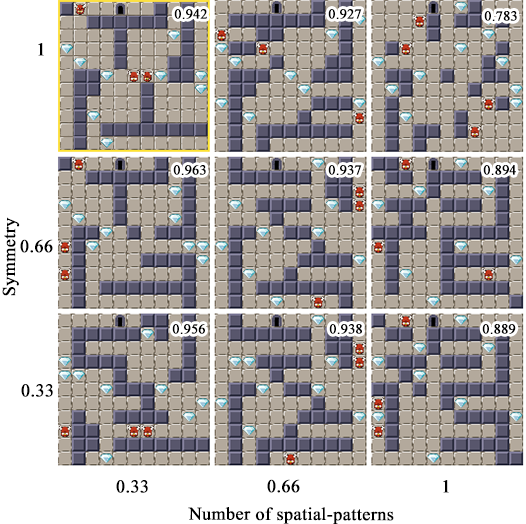
\includegraphics[width=0.49\textwidth]{figures/ICMAPE-figs/figure5.png}
     }
     \hfill
     \subfloat[]{%
       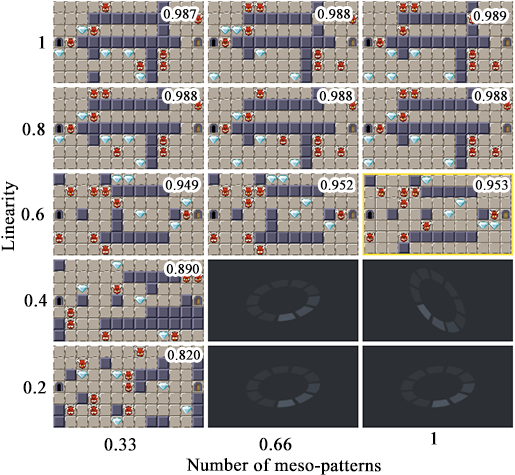
\includegraphics[width=0.49\textwidth]{figures/ICMAPE-figs/figure8.png}
     }
    
    \caption{Example of direct encoding}
    \label{fig:MAPEGrid1}
\end{figure}

As highlighted, behavioral feature dimensions are one of the main components of~\acrshort{mape} and all of its variations. They are context-dependant similar to fitness functions with the caveat that they are only used to categorize and place individuals in cells. The features currently available in our implementation of~\acrshort{icmape} in~\acrshort{edd} are presented in table~\ref{table:mape-dimensions} along with a description of each dimension, and an example of each dimension and multiple cells in each dimension in shown in figure~\ref{fig:dimension-examples}. 
% While they are all related to the context of dungeon and adventure games, there are two dimensions, \emph{similarity} and \emph{inner similarity}, which adapts dynamically to the current, i.e., at different time-steps, it will yiled

\begin{table}[h]
\centering
\caption{Developed game based features used as dimensions in the~\acrlong{icmape}}\label{table:mape-dimensions}
% \resizebox{\textwidth}
% \resizebox{\textwidth}
\begin{tabularx}{\textwidth}{|c|X|}
\hline
\rule{0pt}{12pt}
Feature&Definition\\ \hline
% \\[-6pt]
Similarity & Refers to the aesthetic (tile-by-tile) similarity between a room and the current designer's design.\\ \hline
Inner Similarity & Refers to the similarity of the sparsity and density of the different tile types of a room designer's current design.\\ \hline
Symmetry & Refers to the aesthetic symmetry of a room.\\ \hline
Leniency & Refers to how challenging rooms are; calculated based on the position of enemies and balance between enemies and treasures.\\ \hline
Linearity & Refers to the amount of paths connecting doors within a room; calculated based on how many spatial patterns are traversed.\\ \hline
\#Meso-Patterns & Refers to the number of meso-patterns that exist within a room, normalized by an estimated maximum number based on the room's size and the minimum chamber size.\\ \hline
\#Spatial-Patterns & Refers to the number of spatial-patterns that exist within a room, which can be chambers, corridor, turns, junctions, and intersections.\\ \hline
\end{tabularx}
\end{table}


% we have also feature dimensions that are dynamic
% only using pair of dimensions that can be interacted and changed by the desinger 
% adapting the behavior space based on the new dimensions that define the dimensions of the space

% by adapting and updating the fitness function based  




% Through this, the designer is effectively reshaping the behavioral dimensions in the search space, where e characteristics where encountered individuals in the search space will be retained 





Finally, Mouret and Clune discuss that a traditional single-objective approach could reach as good fitness in an individual for some of the tasks they experimented~\cite{Mouret2015}. Nevertheless, 1) this would only focus on obtaining one high-performing individual, 2) the search would focus in fewer places of the generative space, and as a consequence, 3) the diversity of the generated individuals would be scarce. The nature of our mixed-initiative tool not only requires but fosters the identification of multiple solutions that would satisfy similar constraints e.g. a linear room could be one with narrow corridors connecting doors or a simple open chamber containing all doors. Therefore, a rich, diverse, and high-performing set of levels to be suggested to the designer that could be generated in a short period, and that is able to adapt to changes over time, is a key necessity for~\acrshort{edd}, and essential feature of~\acrshort{icmape}, the motivation for developing~\acrshort{icmape}.


\begin{figure}[!h]
\centerline{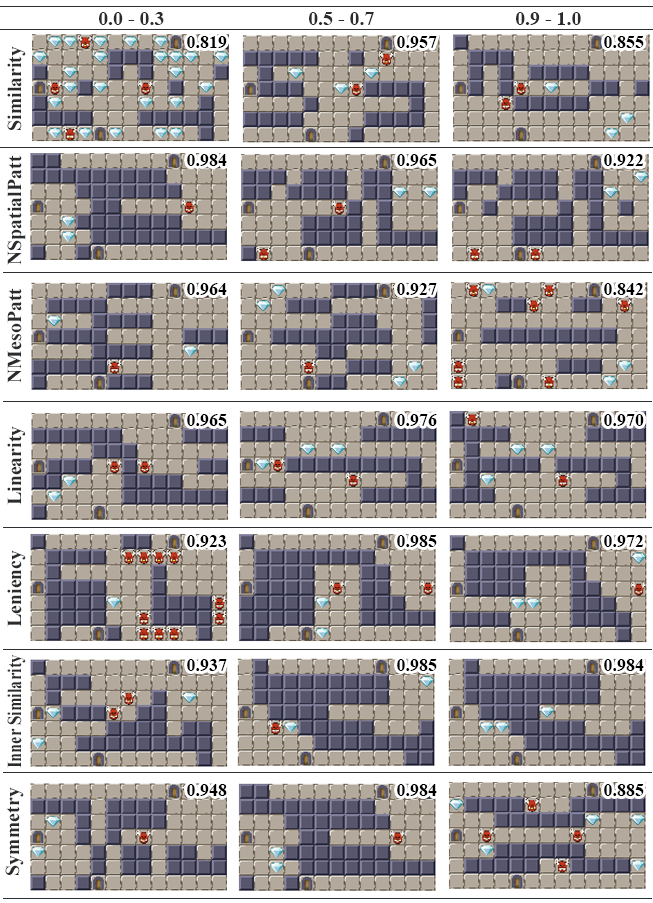
\includegraphics[width=0.7\textwidth]{figures/ICMAPE-figs/figure-all-dimensions-final.png}}
\caption{Example of Elites generated using IC MAP-Elites. Each row represents an independent run of the algorithm using the dimension specified to the left. Each column splits the dimension score into three intervals: 0.0-0.3 (low), 0.5-0.7 (medium), and 0.9-1.0 (high). Each cell displays (top-right) the fitness of the optimal individual in its related interval} \label{fig:dimension-examples}
\end{figure}

% Our fitness function being adaptable

%  this would only focus on obtaining one high-performing individual, 2) the search would focus in fewer places of the generative space, and as a consequence, 3) the diversity of the generated individuals would be scarce. T

% explores the behavioral space for a collection of solutions that are both high-performing and diverse among each other, with the caveat that~\acrshort{mape} discretises the behavior space as a grid of cells informed by a set of feature dimensions that illuminate the behavior space.

\subsection{Machine Learning}
% \begin{itemize}
%     \item Introduce Machine Learning \checkmark
%     \item strategies to train, supervised, unsupervised, reinforcement, self-supervised \checkmark
%     \item Perhaps some interesting work in PCG via ML to discuss more in-depth (but this should be if anywhere in the background). It can be here but very short :D
% \end{itemize}

\acrfull{ml} is a sub-field of~\acrshort{ai} that focuses on using learning algorithms that are able to learn from data and that are trained through some strategy such as supervised learning or reinforcement learning~\cite{Goodfellow2016-DeepLearning}. Formally (and generally), learning in~\acrshort{ml} was operationally defined by Mitchell~\cite{Mitchell97-ML} as: “A computer program is said to learn from experience \textit{E} with respect to some class of tasks \textit{T} and performance measure \textit{P}, if its performance at tasks in \textit{T}, as measured by P, improves with experience \textit{E}.” 

The task~\textit{T} in~\acrshort{ml} is not the learning \textit{per se}, rather learning is the way to attain the ability to solve the tasks.~\acrshort{ml} helps us solve complex tasks that are deemed to complex to be solver by fixed programs such as the creation of games~\cite{summerville2018procedural} or playing games~\cite{Mnih2015-AtariDeepRL,Justesen2020-DLGamePlaying}. Tasks in~\acrshort{ml} might be a \emph{classification} task: what category \textit{k} an input belongs~\cite{Clanuwat2019-Kuronet}; a \emph{regression} task: where it is asked to predict some numerical value based on some input~\cite{regressiontask}; \emph{synthesis} task: create new examples based on the training samples~\cite{torrado2019-bootstrappingGAN}; or \emph{machine translation} task: translate an input from one language to another~\cite{Hartmann2019-UnsupervisedWordTranslation}.

Moreover, performance~\textit{P} relates to how a learning model is assessed to check that it is actually learning from experience~\textit{E} to tackle task~\textit{T}. Depending on the type of task that the model must solve, the performance measure would vary, as it is dependant on it, similarly as to how fitness functions are dependant on the problem to be solved. The usual performance measures used are \textbf{accuracy} and \textbf{error rate}. For tasks such as image generation the \textbf{inception score} is normally used~\cite{Salimans2016-InceptionScore} or for machine translation the \textbf{BLEU} is used to measure the quality of the translated text~\cite{Papineni2002-BLEU}. The key aspect when evaluating performance in a task, is that the learning model should be tested with data it has not used for learning; thus showing the ability of the model to solve "unknown" tasks~\cite{Goodfellow2016-DeepLearning}. 

Furthermore, experience~\textit{E} is related to the data and examples provided to the tool and what strategy is used to train a learning model. Learning strategies in~\acrshort{ml} can be categorized in two main learning strategies: \emph{Supervised} and \emph{Unsupervised} learning. However,~\acrfull{rl} has gain monumental interest from the research community, and is the current learning strategy that is used to solve many tasks due to the metaphor regarding how human's learn and the fact that the learning happens by experiencing the environment rather than learning the data~\cite{Juliani2019-obstacleTower}.~\acrfull{ssl} has also been gaining popularity as an approach to move away from traditional supervised training by not using human annotated dataset to learn representations of data~\cite{Doersch2017-ssl}. 

%%Discuss 
% Over the past years,~\acrshort{ml} has gain popularity in the field of~\acrshort{pcg} in what is called~\acrshort{pcg} via~\acrshort{ml}~\cite{summerville2018procedural}. 
% ~\acrshort{pcg} via~\acrshort{ml} is a prospect area that have shown exciting results for generating a vast amount of game content. Yet creating game levels~\cite{Snodgrass17-GenerateMapsMArkovModels}  for approaches 
% Approaches using supervised learnin
% With datasets such as the Video Game Level Corpus~\cite{Summerville2016-vglc}, many approaches have been 

\subsubsection{Designer Preference}

To explore designer modeling and it's benefits, it was proposed the designer's preference model to drive the content generation in~\acrshort{icmape}~\cite{Alvarez2020-DesignerPreference}. In this work, the suggested~\acrshort{mape} grid is used to compose a dataset that is used as an estimator of the designer's preferences. The goal and motivation of modeling the designer's preferences was to use a surrogate model that could capture the subjective evaluation of the designer together with an objective evaluation from the fitness function. The model, the training, and the usage is depicted in figure~\ref{fig:desPrefModel}. 

\begin{figure}
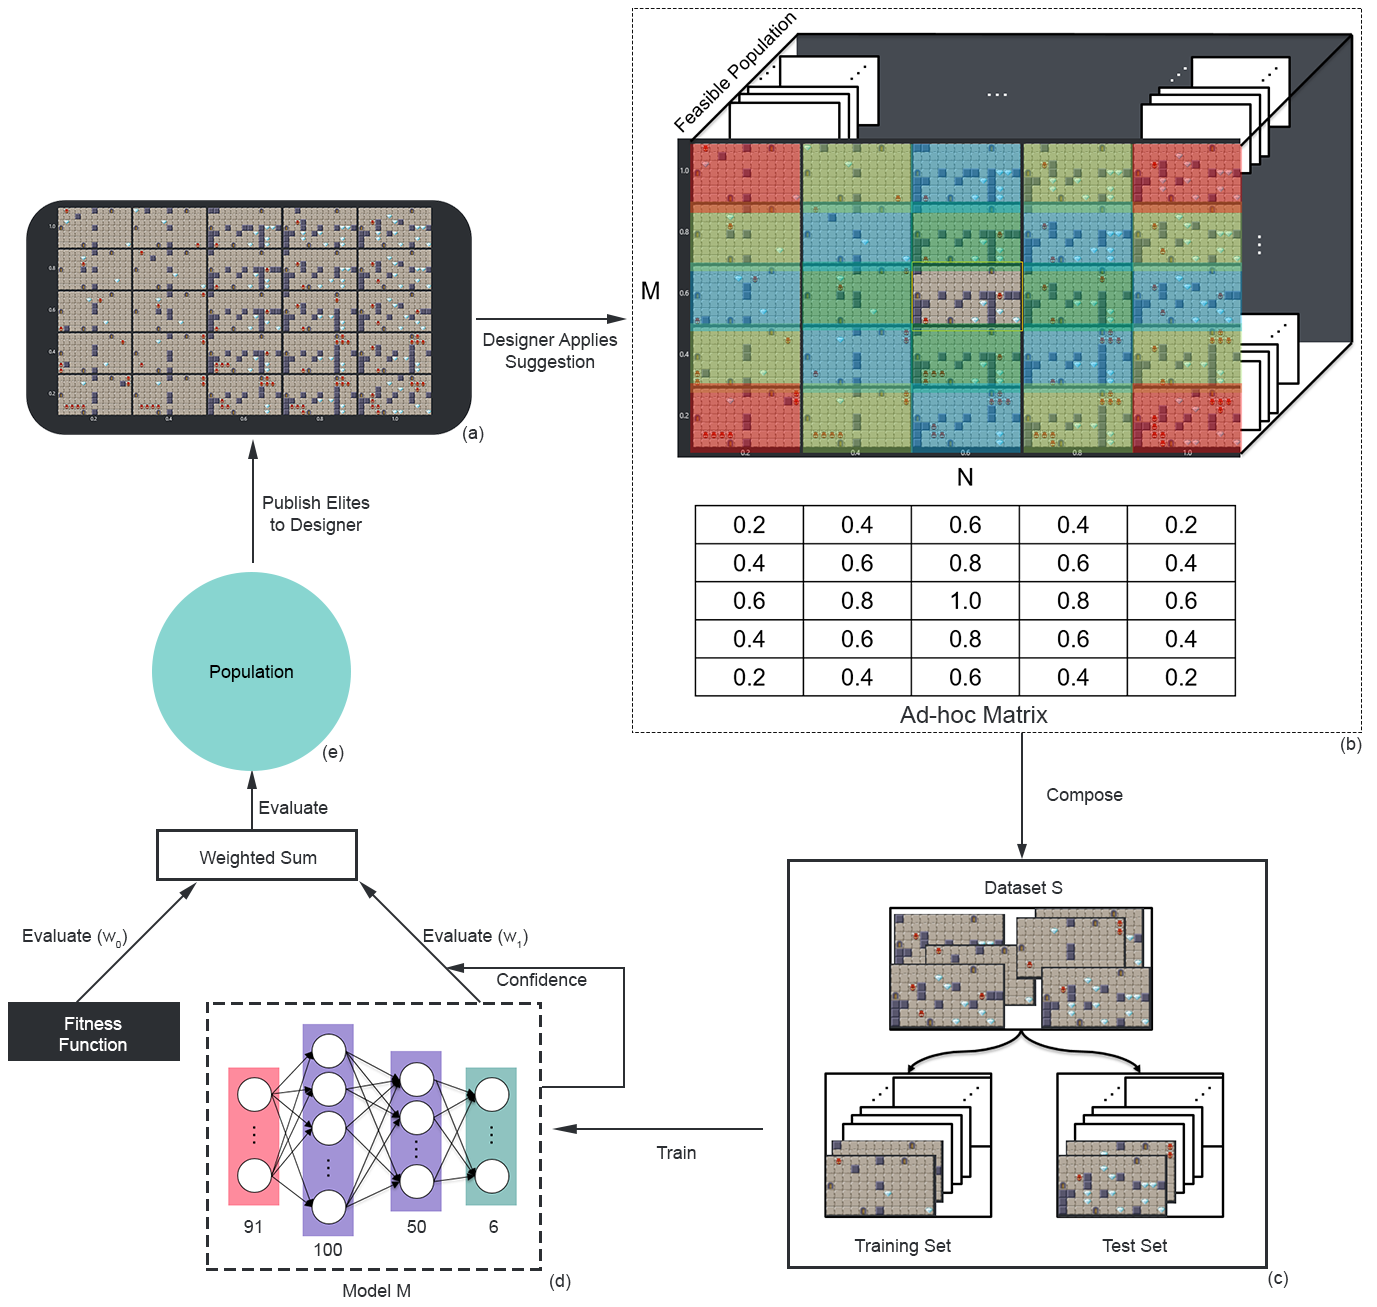
\includegraphics[width=\textwidth]{figures/DesPref-figs/desPrefModel.png}
\caption{Overview of the Designer Preference Model integrated into the fitness function of EDD. Elites are published and shown to the designer in a grid fashion (a), and once the designer chooses and applies one of the suggestions, an ad-hoc matrix is created based on the position of the selected suggestion to estimate the preference of suggestions (b). The ad-hoc matrix is then applied to all the elites in the grid, and the feasible populations within the EA cells to compose a general dataset $S$ with rooms labeled by the estimated preference. The composed dataset $S$ is then subdivided into a training set (90\%) and test set (10\%), both with the same label distribution (c). The dataset is used to train a model $M$, which is a relatively small neural network, for 20 epochs (d). The  model is then used to evaluate the population of the EA together with the current fitness function in a weighted sum, with the weight of the model $M$ conditioned by the confidence of the network (e).} \label{fig:desPrefModel}
\end{figure}

Following a proactive learning approach~\cite{donmez2008proactive}, whenever the designer chooses some suggestion, the system trained a learning model $M$ (i.e. a neural network) with a new set of preferred content (dataset $S$) using the current suggested cells and their population. The result was an adapted model similar to the work by Liapis et al.~\cite{Liapis2012-adaptiveVisual}, which learned overtime the designer's preferences in relation to their choices. Once the model is trained, it is incorporated in the evolutionary loop to drive evolution by means of evaluating the content in a weighted sum with the fitness function. The model slowly fits towards the designer’s preference, and as it's predictions become more confident, the more weight $W_{1}$ it has in the final evaluation. Confidence is calculated based on the output of the softmax layer, which can be interpreted as probabilities for each class. The evaluation resulted in the weights (Eq.~\ref{eq:weights}) and the final weighted sum (Eq.~\ref{eq:weightedSum}).

\begin{equation} \label{eq:weights}
\begin{split}
 w_{1}={}&\min(M_{conf} \cdot M_{TestAcc}, 0.5),\\
w_{0} ={}& 1.0 - w_{1}   
\end{split}
\end{equation}

\begin{equation} \label{eq:weightedSum}
weightedSum = (w_{0} \cdot objective) + (w_{1} \cdot predicted_{pref})
\end{equation}

We evaluated the model and its usability in a user study with fifteen game design students. The results while not significant as there was not enough data to demonstrate the advantage of the model; it allowed the analysis of system's challenges. These challenges where presented as three open areas for active research: \textit{Dataset}: the type and amount of data collected; \textit{Preference modality}: what represents preference in the design and creative process; and \textit{Dynamic-Dynamic System vs. Dynamic-Static System}: the competing properties of a dynamic learning environment, e.g., a designer that traverse the design space, with a dynamically adapting model, e.g., a learning model that tries to adapt as the designer traverse the design space, and it's trade-offs.

\subsubsection{Style Clustering and Designer Personas}

% \begin{itemize}
%     \item Introduce a bit on personas, and on style modeling (I need to check my other computer where i have most of the related work on the topic)
%     \item the main thing here is to discuss the work on the designer personas. use the figures from the paper and such on
% \end{itemize}

\begin{figure}
\centerline{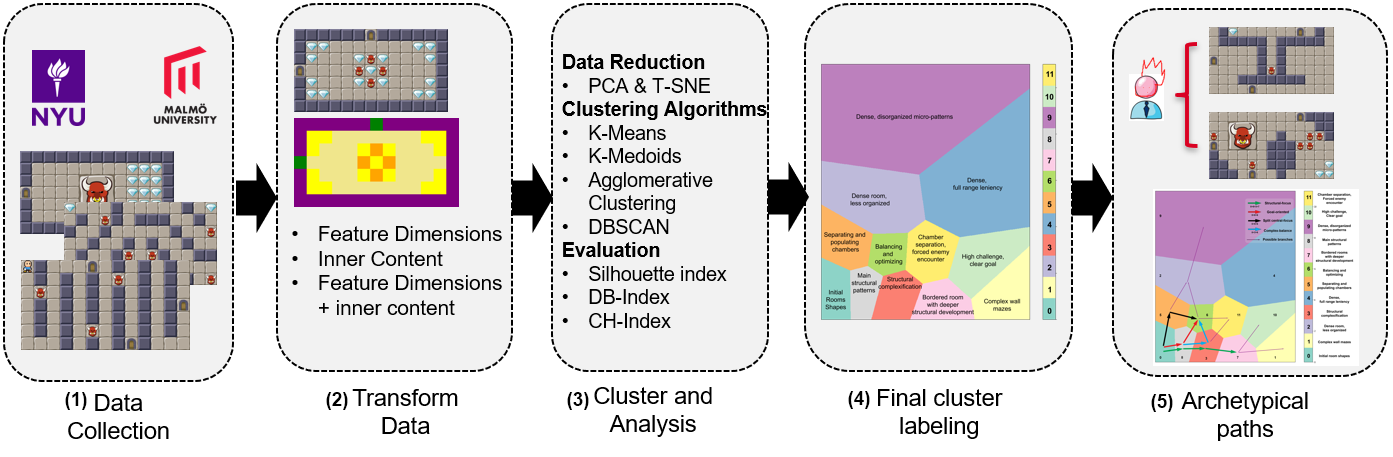
\includegraphics[width=\textwidth]{figures/DesPersonas-figs/process-steps.png}}
\caption{The stages of the design style clustering development: (1) Data was first collected through two user studies. (2) Then, using the design sequences, the data was processed into five different datasets, one using the room images, a second using the tiles information, and three using tabular information. (3) A data reduction technique was applied to different datasets, and then they were clustered and internally evaluated. (4) The clusters were formed, picked from the best performing methods, and labeled based on the data points within each cluster. The cluster were evaluated by visualizing how a typical design session traverse the various clusters, and K-Means (K=12) was chosen as the final approach. (5) Finally, using this final approach all the sequences were clustered and archetypical paths were identified.
} \label{fig:clusteringApproach}
\end{figure}

To further explore designer modeling, it was proposed an alternative approach by clustering designers' design styles~\cite{alvarez2020-designerpersonas}. The basic premise was that by identifying a set of styles that most designers follow when creating content, and model how the designer traverse such a style space, a model that captured the designer's intentions, goals, and style could be created. For instance, rooms for a game like the binding of Isaac~\cite{bindingISAAC} could be classified based on multiple characteristics such as the room's objectives regarding enemies and treasures, access to different areas, or hidden challenges and treasures. Moreover, different designers could reach the same room style through different paths, where the focus along the creation could vary. Some designers would focus on the room's topology before anything else, whereas others would focus first on the objectives a player must achieve. 

\begin{figure}[t]
\centerline{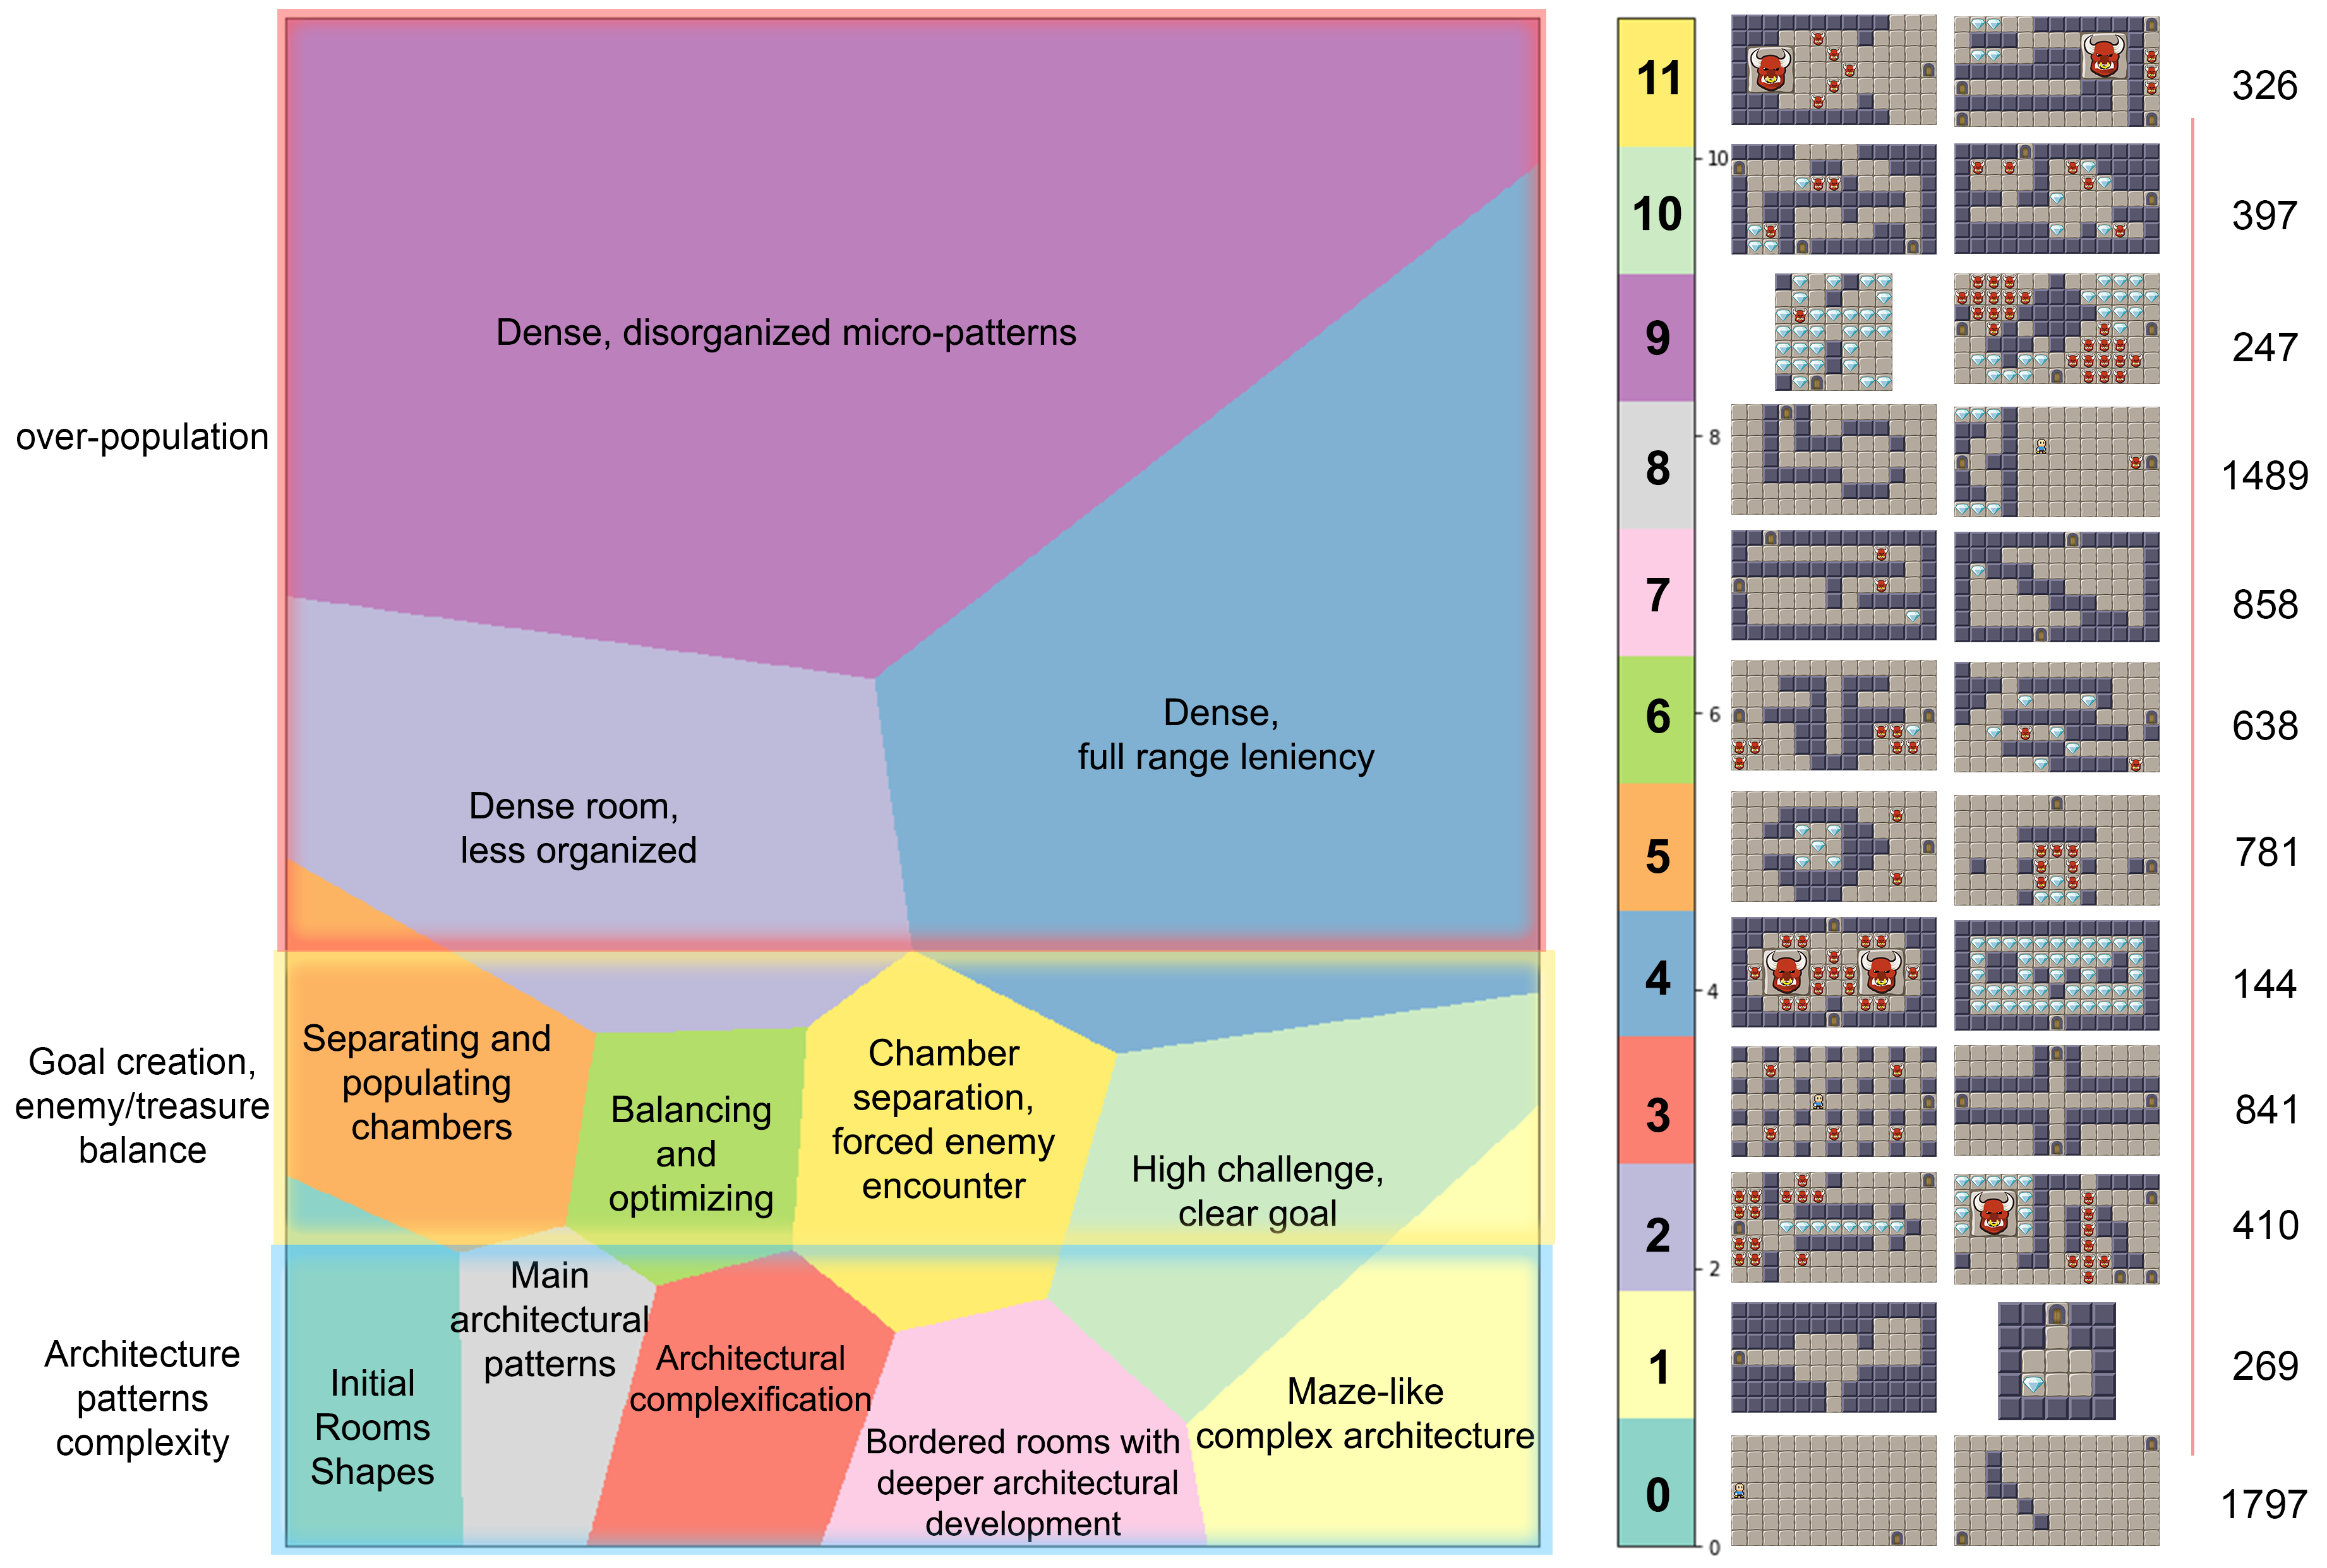
\includegraphics[width=\textwidth]{figures/DesPersonas-figs/final-cluster.png}}
\caption{Best resulting cluster set. K-Means (K=12), using the \textbf{Tiles} Dataset. While it scores slightly less in the internal indices that other setups, a qualitative analysis successfully gives us more granularity by subdividing the main bottom clusters, to label and cluster the design process of designers. Sample rooms belonging to each cluster are displayed on the right, next to the total number of rooms in the cluster.} \label{fig:all-clusters}
\end{figure}

With such as motivation and objective, it was compiled data of designers' designs and the creation process of each individual room in the~\acrshort{edd} to create these models. The data was collected from two user studies, the one documented in the Designer's Preference Model previously described~\cite{Alvarez2020-DesignerPreference} with game design students, and another with practitioners and academic researchers within the computational intelligence in games area. The data was used to create five different datasets that were used in the experiment to analyze multiple variations and possibilities. The datasets were analyzed, experimented on, and compared to obtain the final clusters that effectively divided the design style space. The process is shown in figure~\ref{fig:clusteringApproach}. Figure \ref{fig:all-clusters} shows the final design style clusters with the setup that performed best among all the different experiments (K-Means (K=12), using the \textbf{Tiles} Dataset).

\begin{figure}[t!]
\centerline{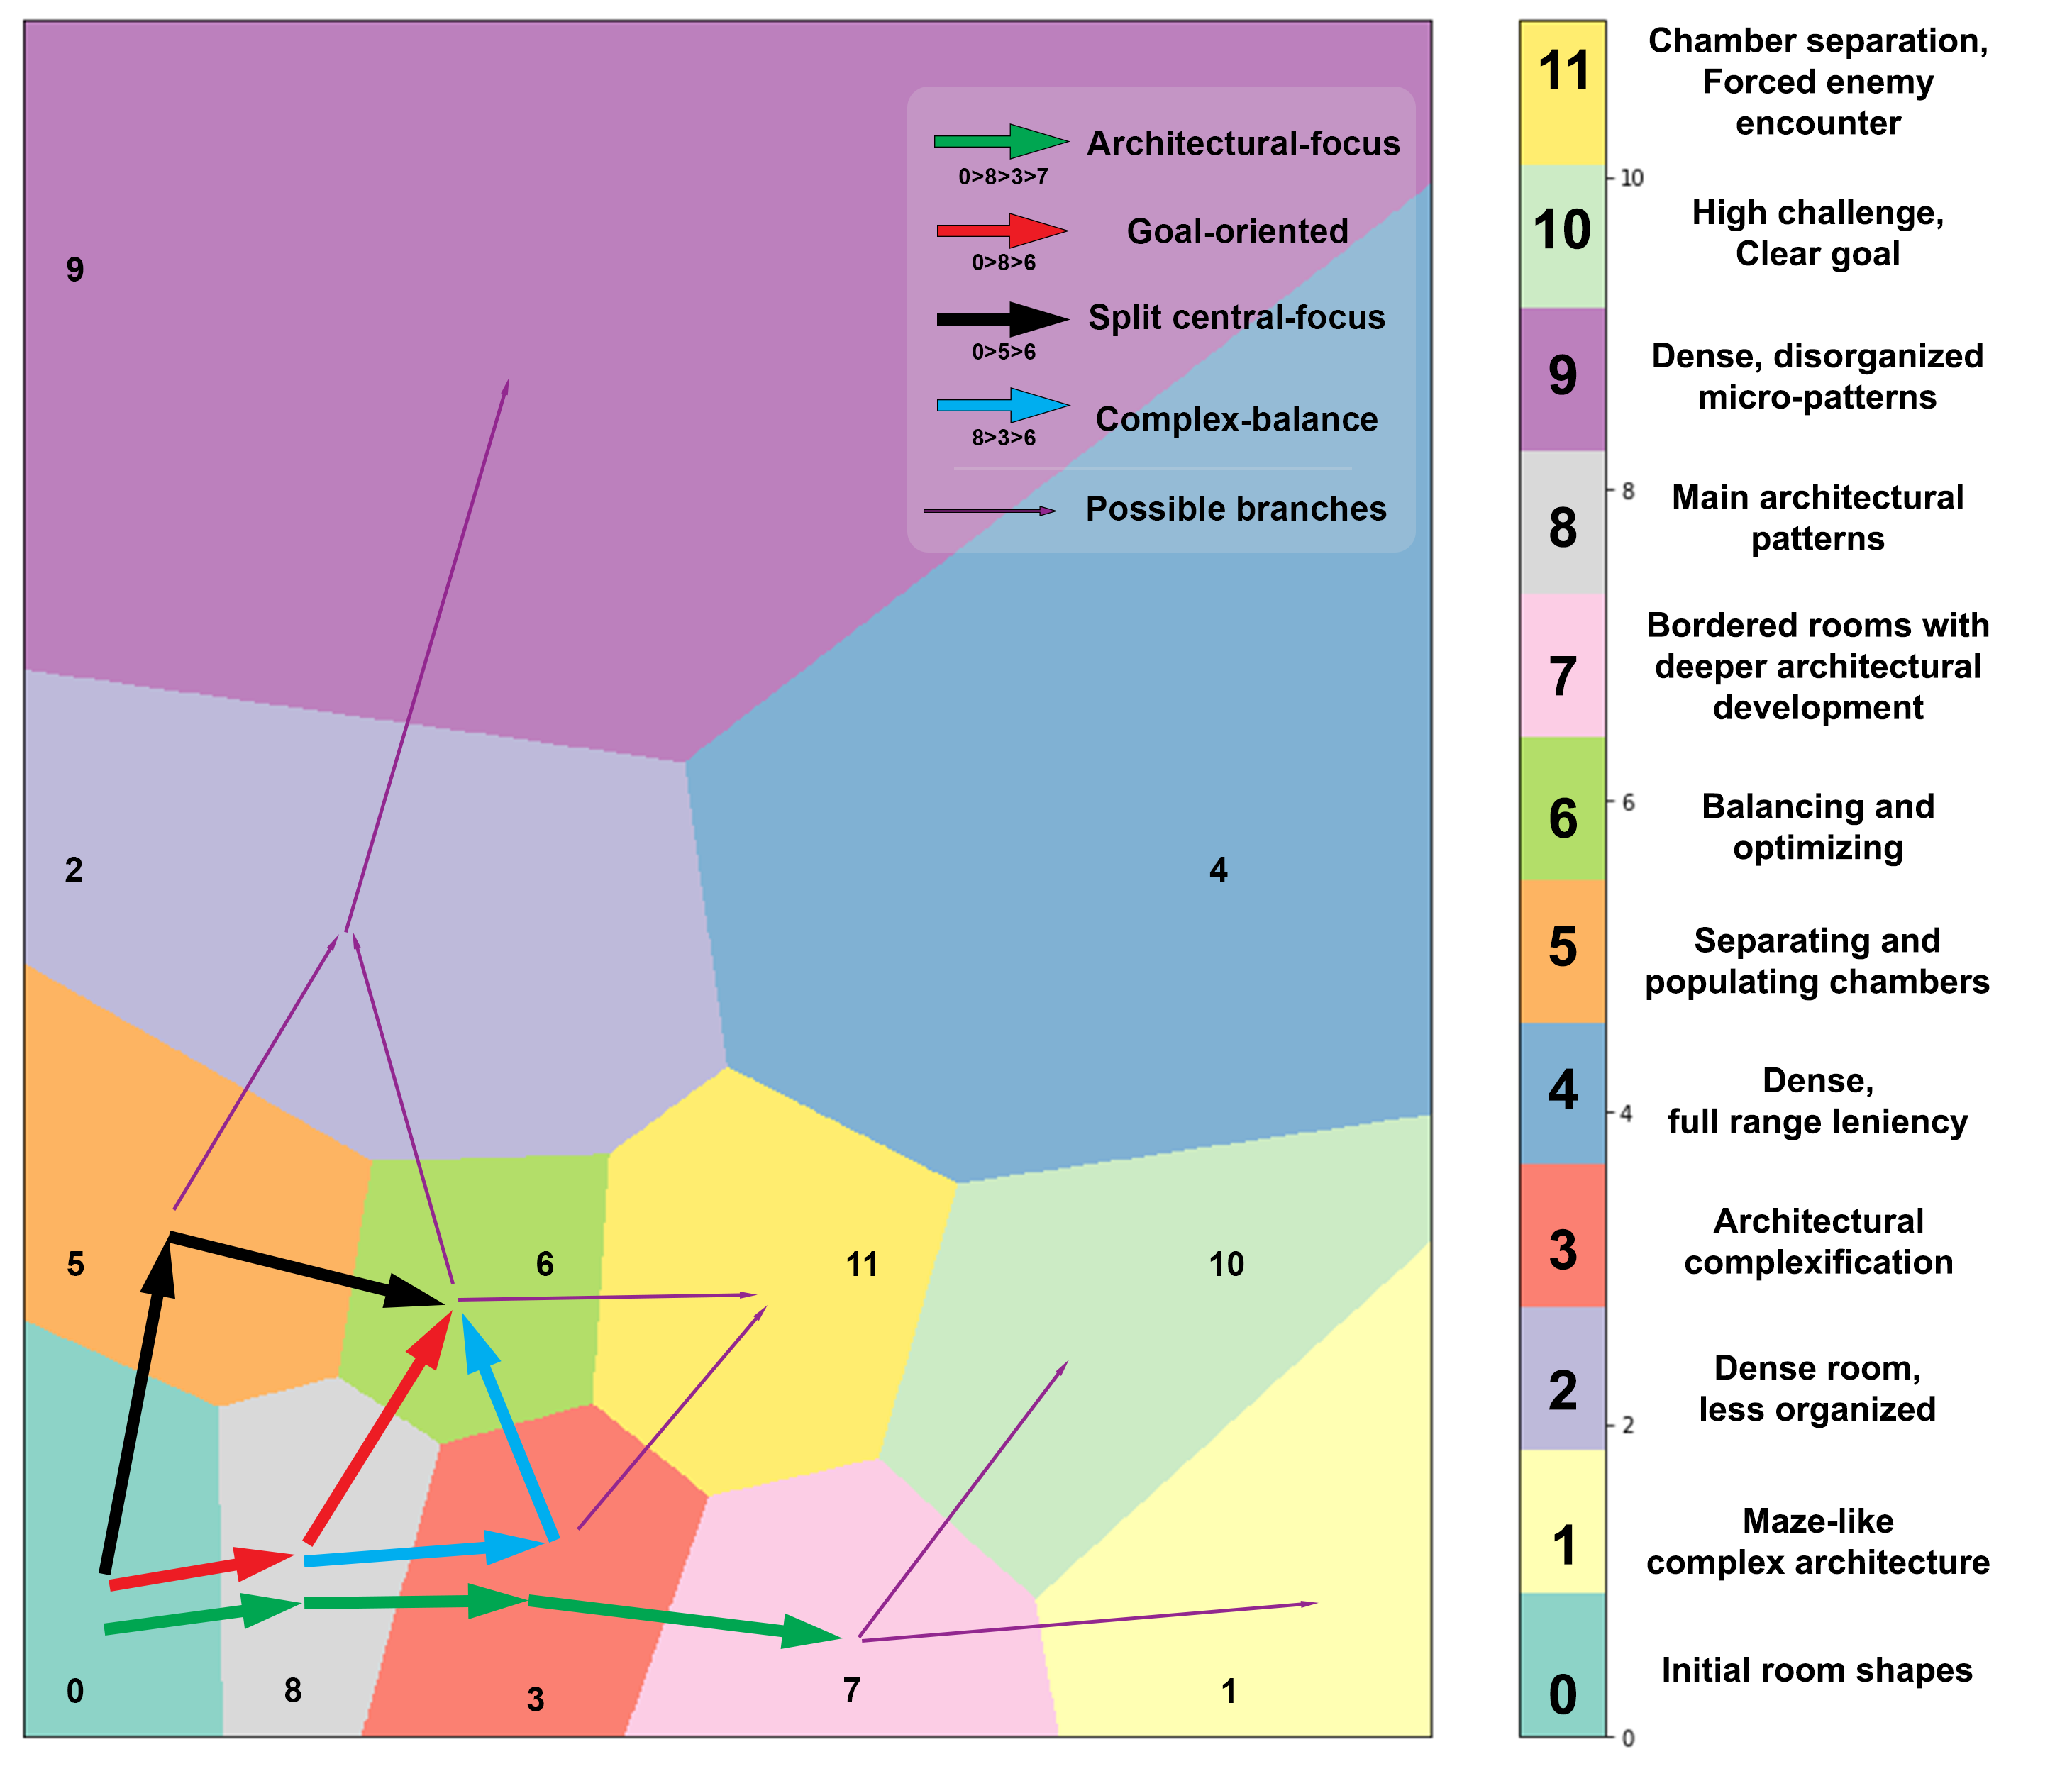
\includegraphics[width=\textwidth]{figures/DesPersonas-figs/resulting-paths-FINAL.png}}
\caption{Final and common designer trajectories. With thick arrows it is presented the archetypical paths, calculated using the frequencies of subsequences from $180$ diverse rooms. Each color represent a unique trajectory; with green the \textsc{Architectural-focus}, with red the \textsc{Goal-oriented}, with black the \textsc{Split central-focus}, and with blue the \textsc{Complex-balance}. Finally, thinner purple arrows extending from clusters traversed by the archetypical paths show the multiple possible branches that an archetypical path can deviate or extend to.} \label{fig:desPersonas}
\end{figure}

Moreover, with the design style cluster, we could then analyzed the design process in function of the traversed clusters rather than evaluating each individual step. To do this, we analyzed the traversed clusters as unique trajectories, and gather the common patterns from the trajectories by applying the Generalized Sequential Pattern (GSP) algorithm, which locates frequent subsequences in the analyzed trajectories. Through this, four \textit{designer personas} were identified. \textit{Designer personas} are defined as archetypical paths through style space that are commonly taken by designers when creating their content. In figure~\ref{fig:desPersonas} it is shown the identified \textit{designer personas}, and figure~\ref{fig:desPersonasExamples} it is presented representative examples per each designer persona.

\begin{figure}[t]
    \centering
     \subfloat[\textsc{Architectural-focus}\label{subfig-1:dummy}]{%
       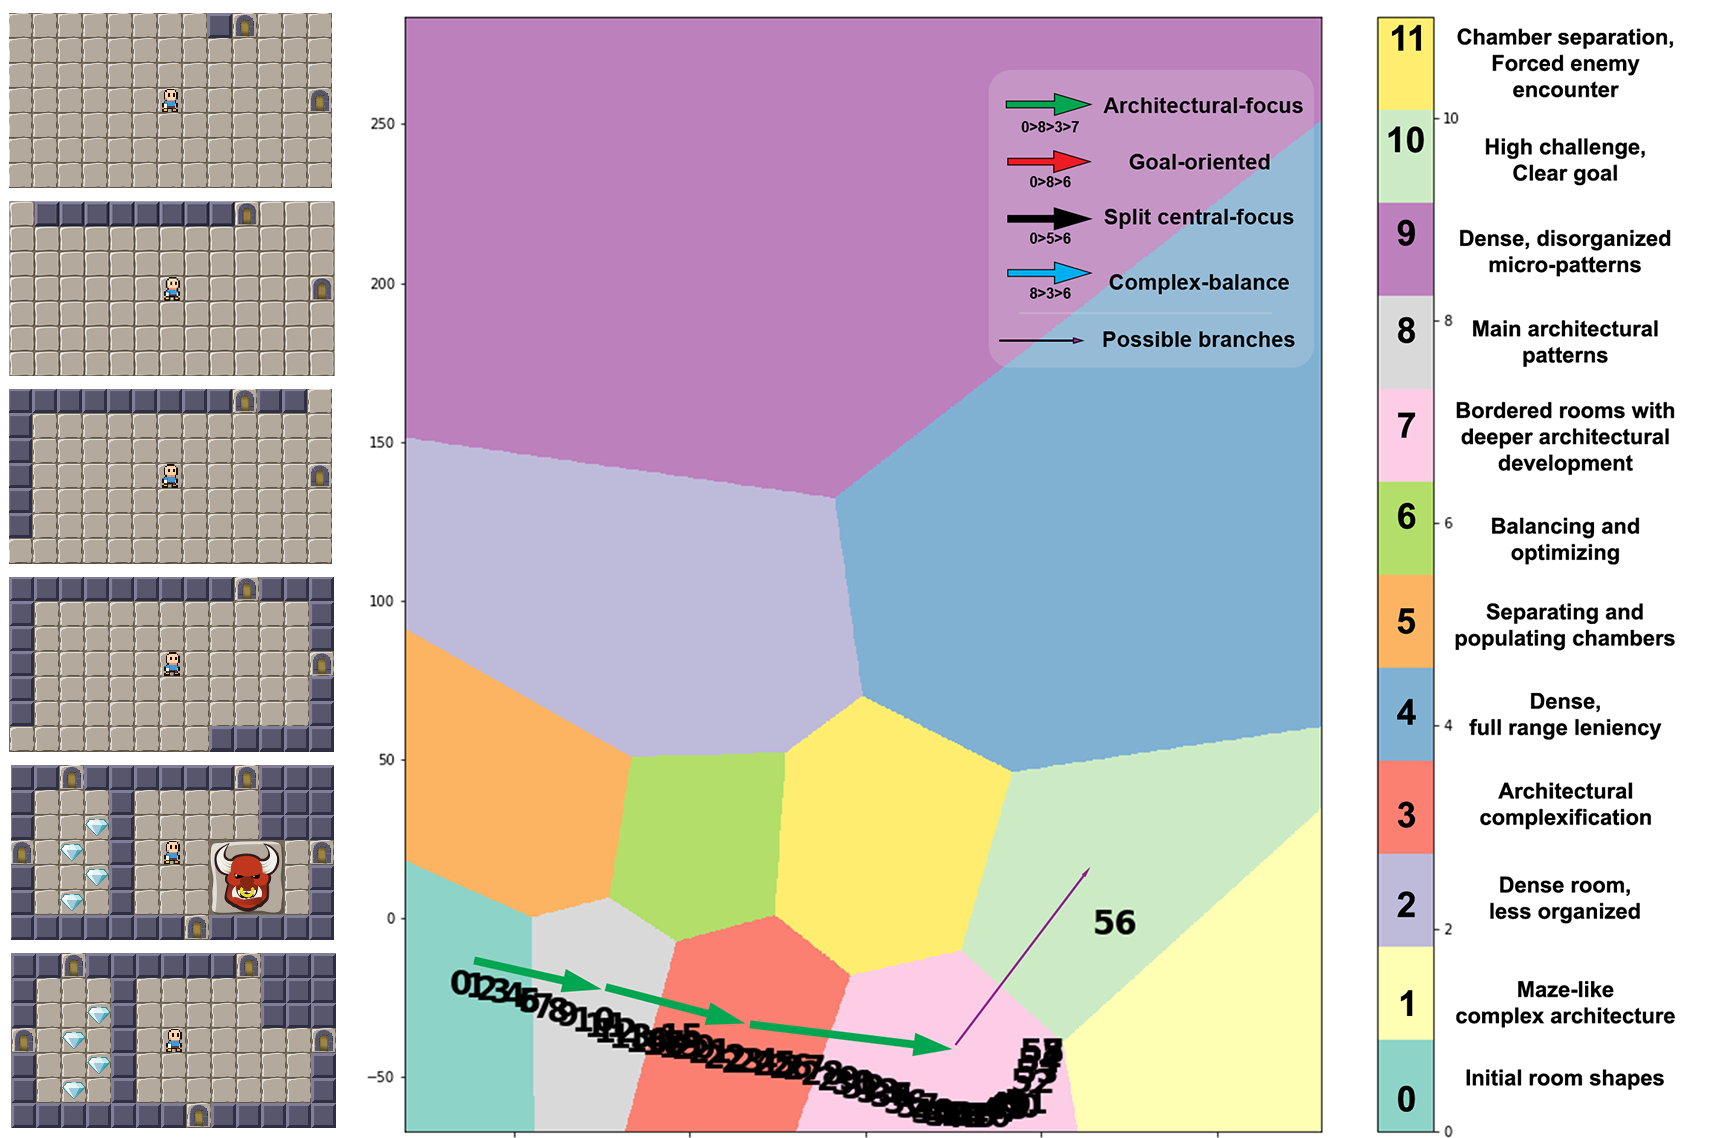
\includegraphics[width=0.6\textwidth]{figures/DesPersonas-figs/1.png}
     }
     \hfill
     \subfloat[\textsc{Goal-oriented}\label{subfig-2:dummy}]{%
       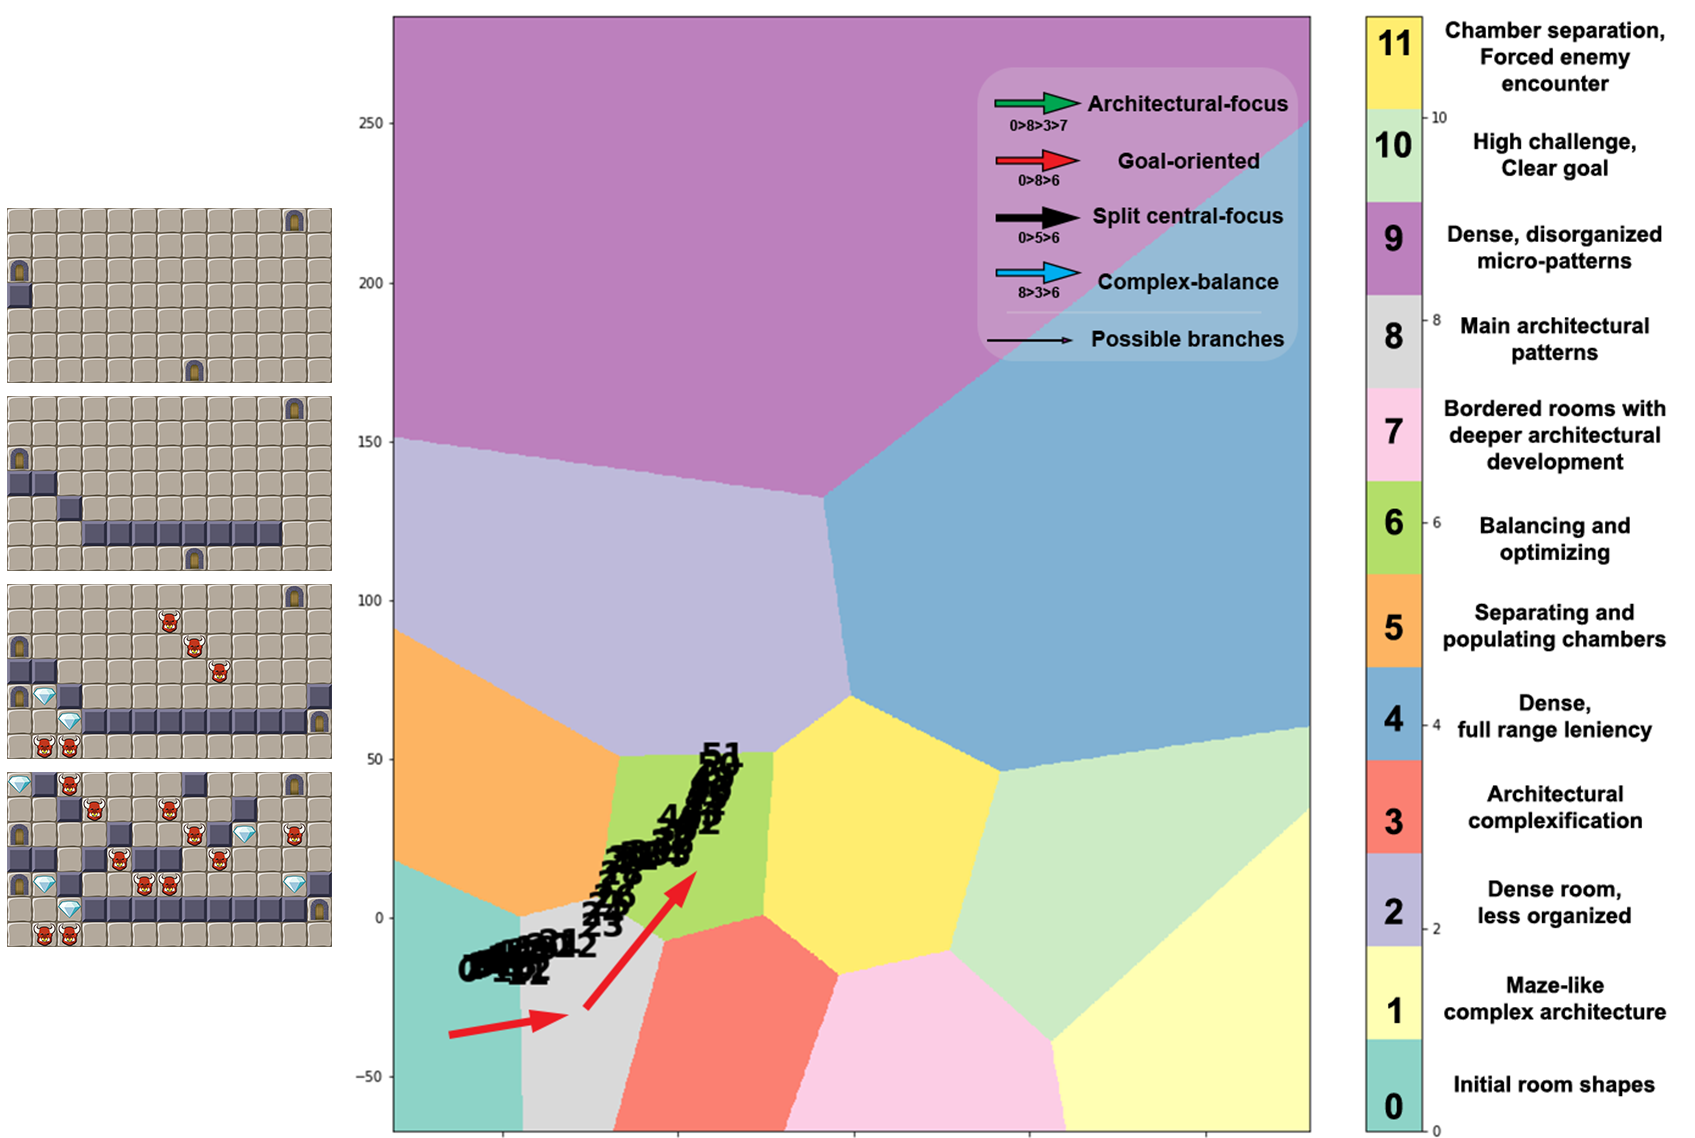
\includegraphics[width=0.45\textwidth]{figures/DesPersonas-figs/2.png}
     }\hfill
    %  \medskip
     \subfloat[\textsc{Split central-focus}\label{subfig-3:dummy}]{%
       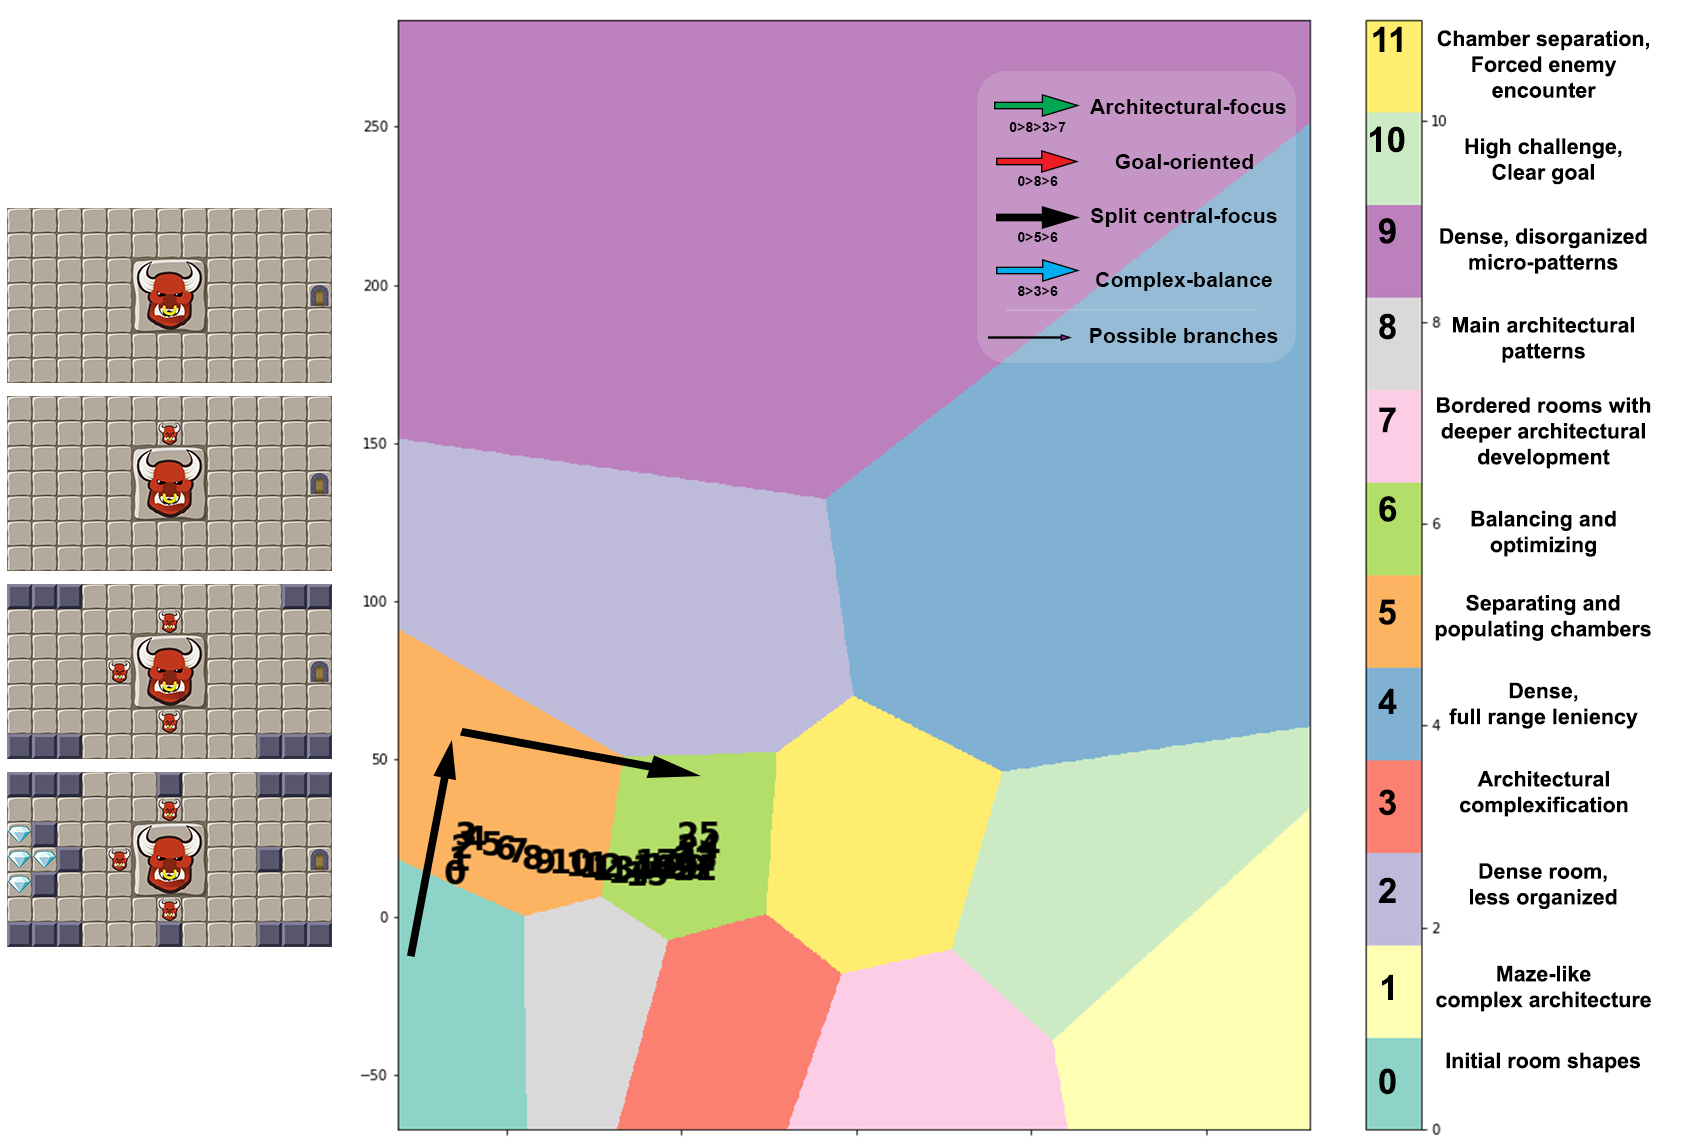
\includegraphics[width=0.45\textwidth]{figures/DesPersonas-figs/3.png}
     }
     \hfill
     \subfloat[\textsc{Complex-balance}\label{subfig-4:dummy}]{%
       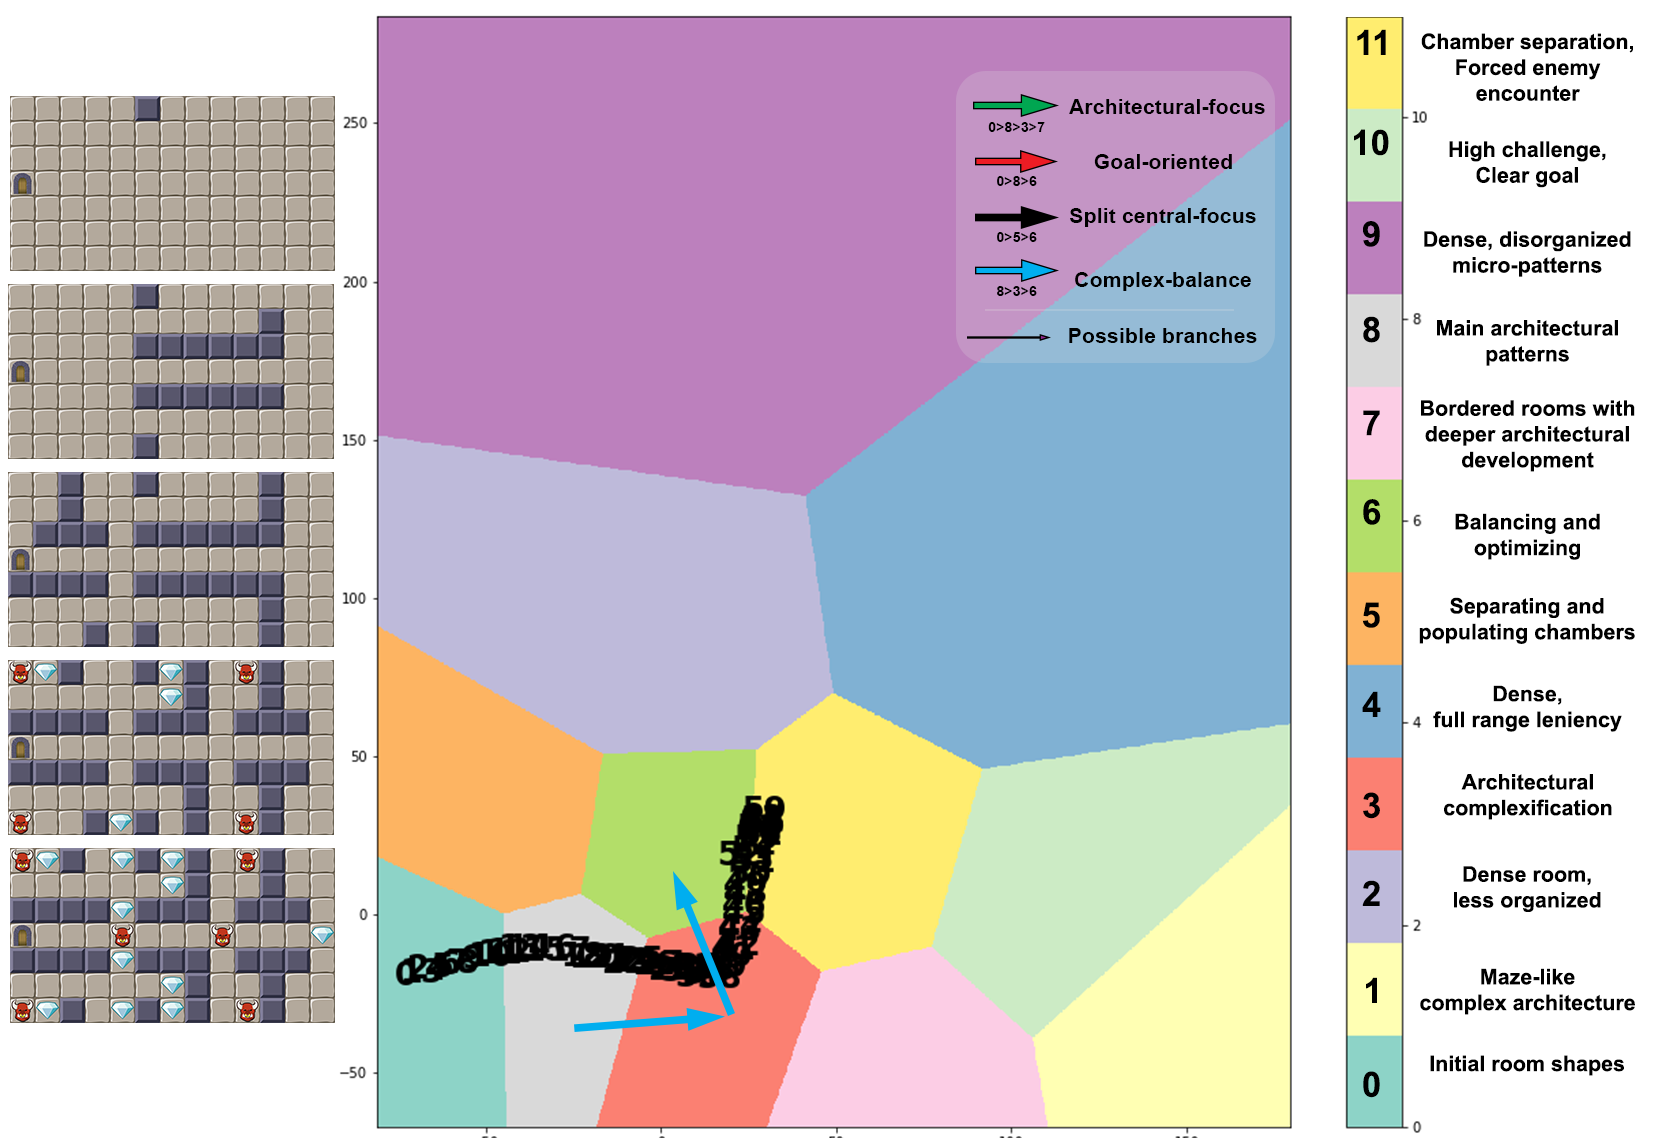
\includegraphics[width=0.6\textwidth]{figures/DesPersonas-figs/4.png}
     }
    
    \caption{Examples of each of the archetypical paths from one of the frequent sequences used to create the clusters. To the left of each subfigure, we present each key step in the trajectory i.e. when the design entered a new cluster. (a) presents the \textsc{Architectural-focus} archetypical path where the focus is firstly on creating the structural design of the rooms; the design process jumps back and forth suddenly to cluster 10 (one of the possible branches) due to the designer adding a boss, and removing it immediately. (b) presents the \textsc{Goal-oriented} archetypical path where the design focus on a minimal structure complexity and mix between adding structural changes and enemies/treasures. (c) shows the \textsc{Split central-focus} archetypical path where, intentionally, the designer creates a center obstacle with a boss and build around it. Finally, (d) presents the \textsc{Complex-balance} archetypical path; the design focuses on building complex, uncommon structures first and then add some goal to it with enemies and treasures, taking advantage of the spaces.}
    \label{fig:desPersonasExamples}
\end{figure}

% These designer models could then be combined with search-based~\cite{Togelius2011} or other procedural generation methods~\cite{khalifa2020-pcgrl,Volz2018-GANevo} to suggest ways of getting to the next design style from the current one. 